\subsection{Mean Voxels Mask}

We plotted the sample images of the brain from three different perspectives, which 
gives us a general sense of our data. Since the raw data is noisy, we averaged our 
data by time and plotted a histogram to check noise 
variance. The dataset contains a lot of signal noise at the outskirt of the 
brain. The signals are correlated across several voxels, because nearby 
brain locations usually have similar response to the task. However, we assume 
that the noise in the data is mostly independent from one voxel to the next. 
Therefore, we reduce the noise by smoothing in space using averaging across the 
independent noise in the voxels. Based on the histogram, we decided to set the 
threshold to 8000 that leaves out most useless information. Then we extracted the 
data points larger than 8000 such that noise variances are removed. Moreover, 
we apply the Gaussian filtering to smooth by 2 standard deviations in all three 
spatial dimensions.

\begin{figure}[!h]
\centering
\begin{subfigure}{.45\textwidth}
  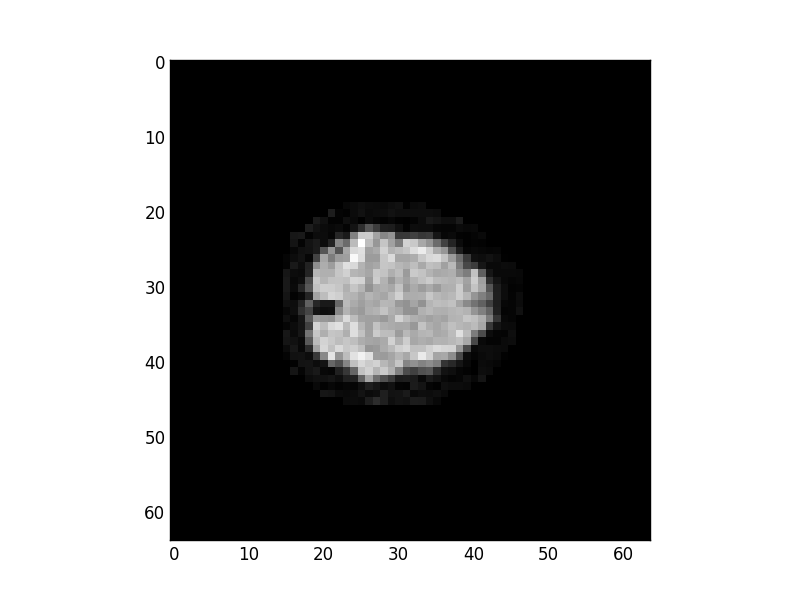
\includegraphics[scale=0.4]{sample_image}
  \caption{Sample Images of Brain}
\end{subfigure}%
\begin{subfigure}{.6\textwidth}
  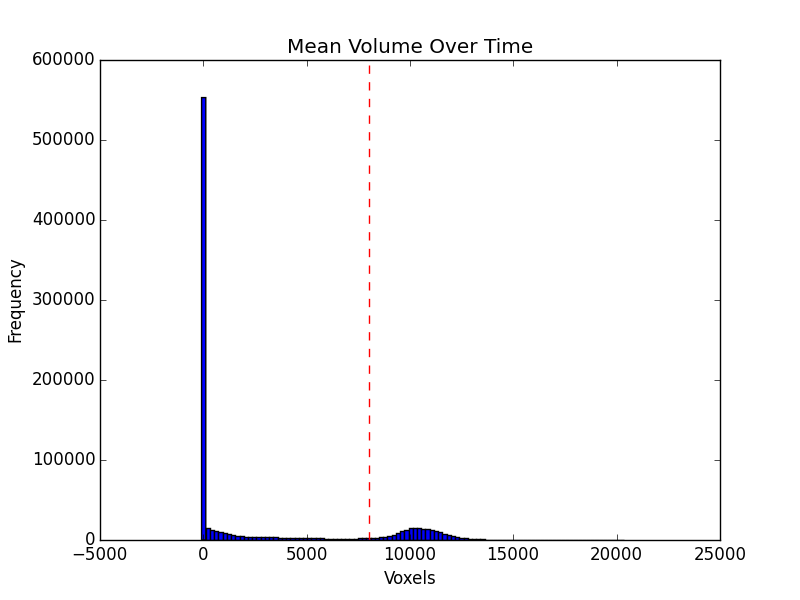
\includegraphics[scale=0.4]{block_mean_data}
  \centering
  \caption{Histogram of Mean of Data}
\end{subfigure}
\caption{Data Preprocessing\label{fig:datapre}}
\end{figure}


